\documentclass[12pt, fleqn]{article}

\usepackage[utf8]{inputenc}
\usepackage[T2A]{fontenc}
\usepackage{amssymb,amsmath,mathrsfs,amsthm}
\usepackage[russian]{babel}
\usepackage{graphicx}
\graphicspath{ {../algoview_106/} }
\usepackage[footnotesize]{caption}
\usepackage{indentfirst}
\usepackage{amsthm}
\usepackage[font=small,labelfont=bf]{caption}
\usepackage[labelsep=space, singlelinecheck=on]{subcaption}

\usepackage{algorithm, setspace}
\usepackage{algpseudocode}
\usepackage[matrix,frame,arrow]{xy}
\usepackage[braket, qm]{qcircuit}
\usepackage[colorlinks=true]{hyperref}
\usepackage{tabularx}
\usepackage{listings}
\usepackage{color}
\usepackage{xcolor}
\usepackage{textcomp}

\textheight=24cm
\textwidth=16cm
\oddsidemargin=5mm
\evensidemargin=-5mm
\marginparwidth=36pt
\topmargin=-1.5cm
\footnotesep=3ex
%\flushbottom
\raggedbottom
\tolerance 3000
\clubpenalty=10000
\widowpenalty=10000
\renewcommand{\baselinestretch}{1.1}
\renewcommand{\baselinestretch}{1.5} 

\addto\captionsrussian{\def\refname{Источники}}
\theoremstyle{definition}
\newtheorem{define}{Определение}
\newtheorem{theorem}{Теорема}
\newtheorem{lemma}[theorem]{Лемма}
\newtheorem{assumption}{Утверждение}

\def\vec#1{\mathchoice{\mbox{\boldmath$\displaystyle#1$}}
{\mbox{\boldmath$\textstyle#1$}} {\mbox{\boldmath$\scriptstyle#1$}} {\mbox{\boldmath$\scriptscriptstyle#1$}}}

\definecolor{mygreen}{rgb}{0,0.6,0}
\definecolor{mygray}{rgb}{0.5,0.5,0.5}
\definecolor{mymauve}{rgb}{0.58,0,0.82}
\definecolor{dkgreen}{rgb}{0,0.6,0}
\definecolor{gray}{rgb}{0.5,0.5,0.5}
\definecolor{mauve}{rgb}{0.58,0,0.82}
\definecolor{gray}{rgb}{0.4,0.4,0.4}
\definecolor{darkblue}{rgb}{0.0,0.0,0.6}
\definecolor{lightblue}{rgb}{0.0,0.0,0.9}
\definecolor{cyan}{rgb}{0.0,0.6,0.6}
\definecolor{darkred}{rgb}{0.6,0.0,0.0}
\definecolor{purple}{rgb}{0.58,0,0.82}


\lstset{
  basicstyle=\ttfamily\footnotesize,
  columns=fullflexible,
  showstringspaces=false,
  numbers=left,                   % where to put the line-numbers
  numberstyle=\tiny\color{gray},  % the style that is used for the line-numbers
  stepnumber=1,
  numbersep=5pt,                  % how far the line-numbers are from the code
  backgroundcolor=\color{white},      % choose the background color. You must add \usepackage{color}
  showspaces=false,               % show spaces adding particular underscores
  showstringspaces=false,         % underline spaces within strings
  showtabs=false,                 % show tabs within strings adding particular underscores
  frame=none,                   % adds a frame around the code
  rulecolor=\color{black},        % if not set, the frame-color may be changed on line-breaks within not-black text (e.g. commens (green here))
  tabsize=2,                      % sets default tabsize to 2 spaces
  captionpos=b,                   % sets the caption-position to bottom
  breaklines=true,                % sets automatic line breaking
  breakatwhitespace=false,        % sets if automatic breaks should only happen at whitespace
  title=\lstname,                   % show the filename of files included with \lstinputlisting;
                                  % also try caption instead of title  
  commentstyle=\color{gray}\upshape
}


\lstdefinelanguage{XML}
{
  morestring=[s][\color{mauve}]{"}{"},
  morestring=[s][\color{black}]{>}{<},
  morecomment=[s]{<?}{?>},
  morecomment=[s][\color{dkgreen}]{<!--}{-->},
  stringstyle=\color{black},
  identifierstyle=\color{lightblue},
  keywordstyle=\color{red},
  caption={\protect\filename@parse{\lstname}\protect\filename@base\text{.}\protect\filename@ext},
  morekeywords={xmlns,xsi,noNamespaceSchemaLocation,type,id,x,y,source,target,version,tool,transRef,roleRef,objective,eventually}% list your attributes here
}

\lstdefinestyle{customc}{
  belowcaptionskip=1\baselineskip,
  breaklines=true,
%   frame=L,
  xleftmargin=\parindent,
  language=C,
  showstringspaces=false,
  basicstyle=\linespread{0.8}\small\ttfamily,
  keywordstyle=\bfseries\color{dkgreen},
  commentstyle=\itshape\color{purple},
  identifierstyle=\color{blue},
  stringstyle=\color{orange},
  caption={\protect\filename@parse{\lstname}\protect\filename@base\text{.}\protect\filename@ext}
}


\newenvironment{packed_enum}{
\begin{enumerate}
  \setlength{\itemsep}{1pt}
  \setlength{\parskip}{0pt}
  \setlength{\parsep}{0pt}
}{\end{enumerate}}

\begin{document}
\hypersetup{pageanchor=false}
% \pagenumbering{Alph} % for correct numbering of document
\begin{titlepage}
\begin{center}
    
\includegraphics[width=58mm]{msu.eps}
    
    Московский государственный университет имени М.В.Ломоносова\\
    Факультет вычислительной математики и кибернетики\\
    Кафедра математических методов прогнозирования\\[25mm]

    \textsf{
        \Large\bfseries 
        Теоретическая работа №1 по курсу <<Суперкомпьютерное моделирование и технологии>>
        \\[5mm] 
        Построение информационного графа и определение свойств заданного фрагмента.
    }\\[12mm]
    
    \begin{flushright}
        \parbox{0.5\textwidth}{
        \begin{flushright}
            \textbf{Выполнил:}\\
            студент 617 группы \\
            Г.В. Кормаков
        \end{flushright}
        }
    \end{flushright}

    \vspace{\fill}
    Москва, 2021
\end{center}

\end{titlepage}
\hypersetup{pageanchor=true}
% \pagenumbering{arabic} % for correct numbering of document
\tableofcontents
\newpage
\section{Постановка задачи}
В рамках выполнения задания был выдан представленный фрагмент программы (Листинг \ref{code:list1}):
\lstinputlisting[language=C, style=customc, label={code:list1}]{../code/program_106.c}{}

Необходимо было выполнить исследование информационной структуры этого фрагмента, рассмотреть связи по операциям, выполняемым в данном фрагменте и определить характеристики, важные для понимания степени параллелизма фрагмента.

Информационную структуру фрагмента необходимо составить на языке разметки Algolang. Для визуализации структуры использовался инструмент Algoview. 
\section{Информационная структура}
Важными для формирования информационной структуры фрагмента показались следующие факты:
\begin{enumerate}
 \item Узлами формируемой структуры являются операторы (чаще всего - это присваивание). Зависимости по данным рассмтривает последовательность обращений в память, однако для оценки информационной структуры более информативным является зависимость по времени исполнения.
 \item При отсутствии зависимостей от предыдущих данных структура фрагмента будет совпадать с описанной ниже, однако если бы перед фрагментом программы присутствовали вычисления, связанные с элементами D[i], то необходимо было бы отразить зависимости в структуре.
 \item Циклические зависимости (например, при присвоении A[i][j] = A[i]][j] + D[i]) не отслеживаются, т.к. по времени нет зависимости между одной и той же областью памяти в явном виде.
\end{enumerate}


Описание информационной структуры приведено ниже на языке Algolang (см. листинг \ref{code:list2}). Для моделирования в среде Algoview параметры были подобраны так, чтобы была возможность рассмотреть структуру.
\lstinputlisting[language=XML, basicstyle=\linespread{0.8}\small\ttfamily, label={code:list2}]{../code/algoload_106.xml}{}

\section{Анализ графового представления}
Представленный в листинге \ref{code:list2} фрагмент был загружен в систему Algoview с собственного профиля. Были получены результаты, скриншоты которых приведены ниже (рис. \ref{fig:XY}, \ref{fig:XZ}, \ref{fig:YZ}  )

\begin{figure}[ht]
\begin{subfigure}{0.5\textwidth}
 \begin{center}
 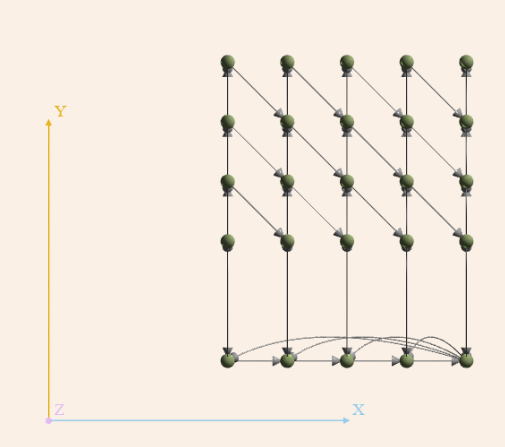
\includegraphics[scale=0.78]{XY_proj.png}
 \caption{Без перспективы}
\end{center}
\end{subfigure}
\begin{subfigure}{0.49\textwidth}
 \begin{center}
 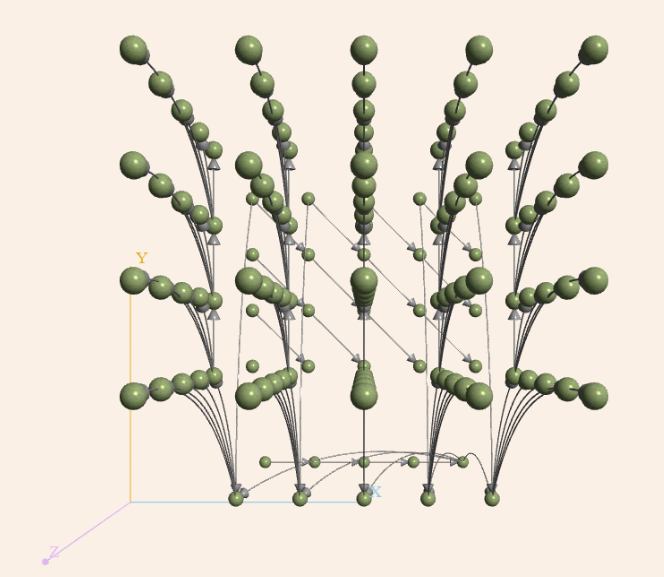
\includegraphics[scale=0.61]{XY_persp.png}
 \caption{С перспективой}
\end{center}
\end{subfigure}
\caption{Проекция на плоскость XY}
\label{fig:XY}
\end{figure}
\begin{figure}[ht]
\begin{subfigure}{0.5\textwidth}
 \begin{center}
 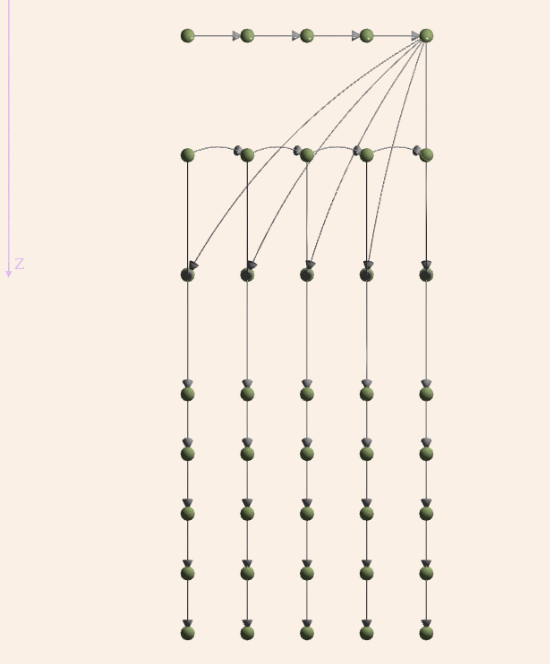
\includegraphics[scale=0.7]{XZ_proj.png}
 \caption{Без перспективы}
\end{center}
\end{subfigure}
\begin{subfigure}{0.49\textwidth}
 \begin{center}
 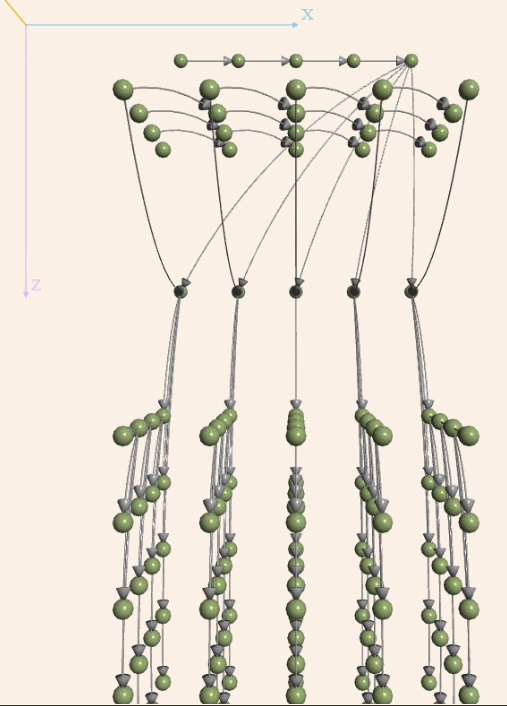
\includegraphics[scale=0.67]{XZ_persp.png}
 \caption{С перспективой}
\end{center}
\end{subfigure}
\caption{Проекция на плоскость XZ}
\label{fig:XZ}
\end{figure}
\begin{figure}[ht]
\begin{subfigure}{\textwidth}
 \begin{center}
 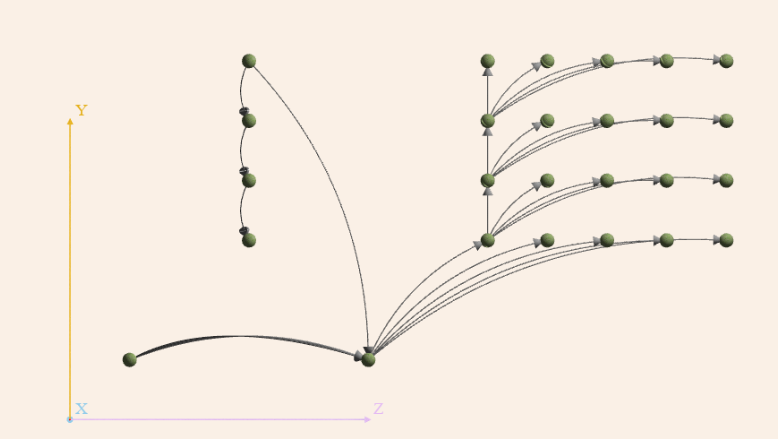
\includegraphics[scale=0.94]{YZ_proj.png}
 \caption{Без перспективы}
\end{center}
\end{subfigure}\\
\begin{subfigure}{\textwidth}
 \begin{center}
 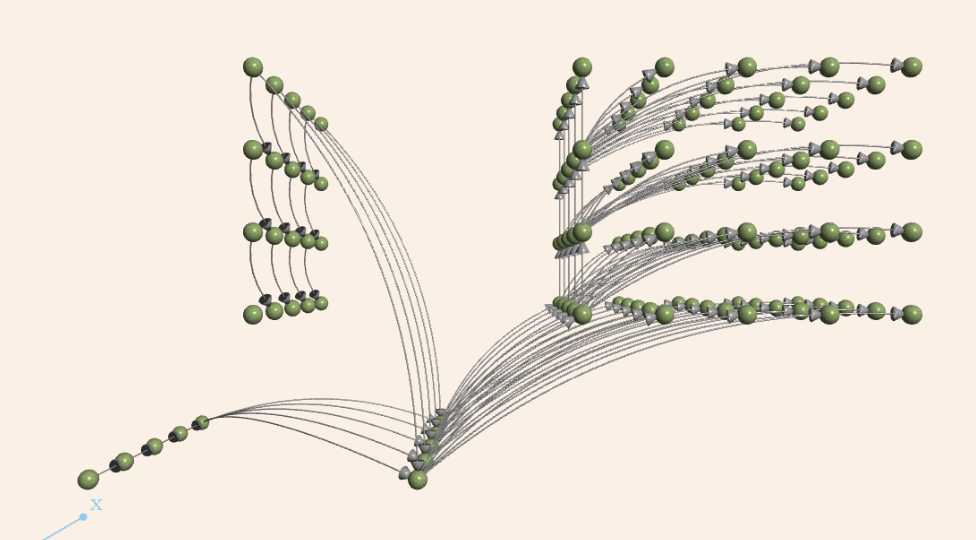
\includegraphics[scale=0.77]{YZ_persp.png}
 \caption{С перспективой}
\end{center}
\end{subfigure}
\caption{Проекция на плоскость YZ}
\label{fig:YZ}
\end{figure}

Наиболее информативной с визуальной точки зрения является проекция на плоскость YZ (рис. \ref{fig:YZ}). Совместим информативное описание фрагмента с рисунком для понимания ресурсов параллелизма и соответсвия с фрагментами (рис. \ref{fig:main}).

Для уточнения зависимостей в цикле размерности 3 используем условие на вторую размерность, как и в приведённом фрагменте листинга \ref{code:list2}. На изображении общими группами отмечены условным образом пути, связанные с зависимостями в циклах. Некоторые из них соответствуют ресурсам параллелизма.
\begin{figure}[ht]
\begin{center}
 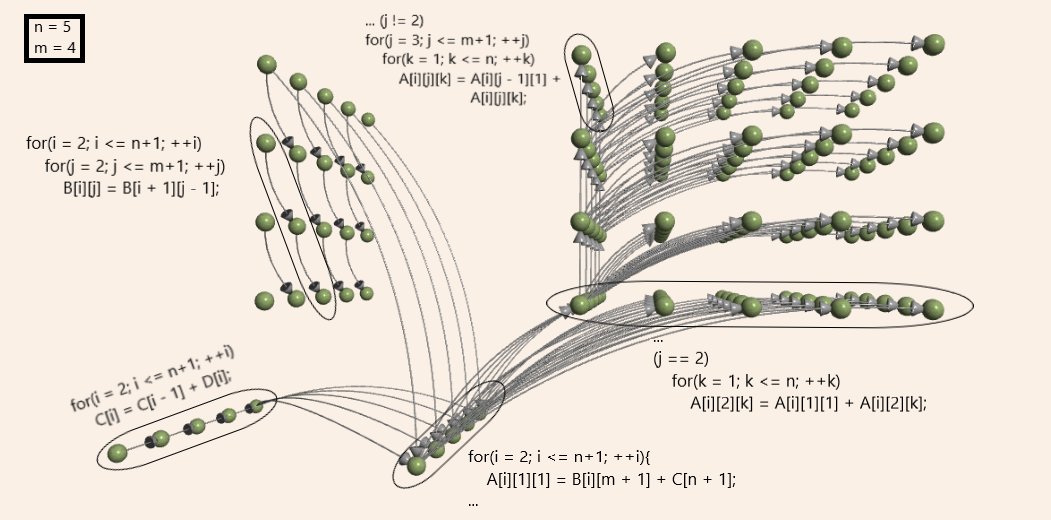
\includegraphics[scale=0.575]{main.png}
 \caption{Комментарии к структуре информационного графа}
 \label{fig:main}
\end{center}
\end{figure}

\section{Сведения об информационной структуре}
Выход алгоритма Algoview: 

Total vertex count: 130, Critical route length: 21, Canonical LPF width: 25
\begin{packed_enum}
 \item \textbf{Последовательная сложность} (число вершин в информационном графе фрагмента). Результата работы программы совпадает с собственными подсчётами. Число вершин=130. 
 В общем случае формула имеет следующий вид: \\ $n + nm + n + nmn = 2n + nm + n^2m = \mathbf{n(nm + m + 2 )} = 5\cdot(20 + 4 + 2) = 130$.
 \item \textbf{Параллельная сложность} (длина (\underline{число дуг}) критического пути в информационном графе). Результат собственных вычислений отличается от результата программы. Результат программы - 21 (не смог найти объяснения, почему результат Algoview такой). Собственный подсчёт - 9. Общая формула собственного подсчёта: $(n - 1) + 1 + (n - 1) = \mathbf{2n - 1} = 9$.

 \item \textbf{Ширина ЯПФ} (максимальное число вершин на ярусе). Результат алгоритма совпадает с собственными вычислениями. Ширина ЯПФ = 25. 
 \textbf{Данная параллельная форма является канонической} (все входные вершины находятся на ярусе 1 и на каждом ярусе k длина максимального пути до любой вершины этого яруса равна k-1). И, следовательно, максимальной (т.е. минимальной высоты).
 
 На рис. \ref{fig:max_lpf} приведён один из ярусов с максимальной шириной. Общая схема подсчёта числа вершин на этом ярусе равна: $\mathbf{n^2} = 25$.
 
 Благодаря ещё одному свойству, критический путь является минимальной из всех возможных высот ЯПФ - 1 (поскольку высота ЯПФ - число вершин). Таким образом, можно подтвердить, что критичекский путь равен 9 для данных параметров (факт взят из знаний предыдущего курса и может быть найден в \cite{Voevodin02}).
 
 \begin{figure}[ht]
\begin{center}
 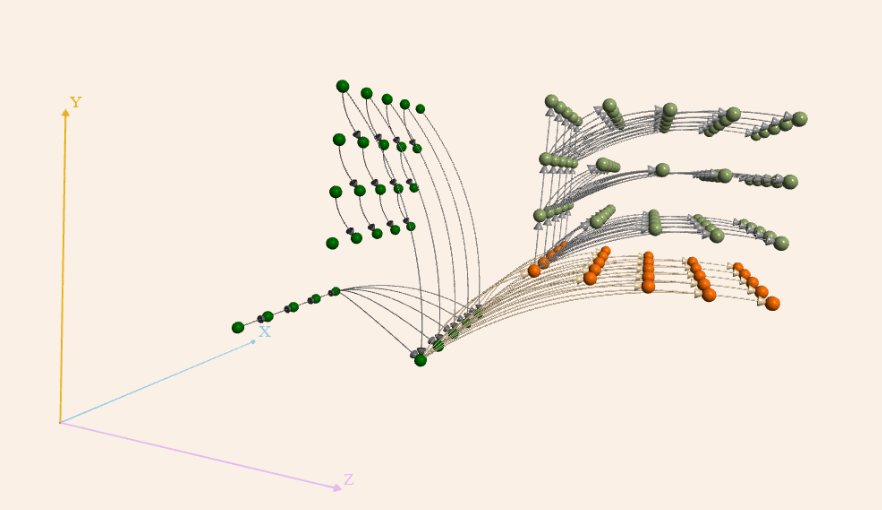
\includegraphics[scale=1]{max_lpf.png}
 \caption{Вид яруса с максимальной шириной (выделен оранжевым)}
 \label{fig:max_lpf}
\end{center}
\end{figure}

 \item \textbf{Максимальная глубина вложенности циклов} = 3.

 \item \textbf{Число различных типов дуг}(тип дуг определяется направляющим вектором и длиной при фиксированных значениях параметров).
 
 Все дуги, имеющие одинаковые направляющие векторы и одинаковую длину, иметют один тип. Если направляющие векторы и длины зависят от внешних параметров, то мы фиксируем параметры.
 
 Стоит отметить, что ранее не рассматривались данные понятия, поэтому интерпретировать данные определения (направляющего вектора и длины) будем по связи с теорией графов и эвристиками...
 
 Направляющие векторы разделим (типизация частично обирается на классификацию in и out из \cite{Voevodin02}) на типы по: 
 \begin{itemize}
 \setlength{\itemsep}{1pt}
  \item Принадлежности входа и выхода дуги одному блоку итераций
  \item Принадлежности входа и выхода дуги одной размерности блока итераций
 \end{itemize} 

 
 В этом случае, по второму критерию отнесения происходит разбиение дуг на типы по входам/выходам в различные размерности. Таким образом, может получиться, что число типов дуг зависит от размерности.
 
 Для приведённого фрагмента типы дуг отчётливо видны на рис. \ref{fig:max_lpf}. \textbf{Всего типов}: 1 + 5 + 1 + 1 + 5 + 5 = 1 + n + 1 + 1 + n + n = \textbf{3(n + 1)} = 18.
 
 \begin{itemize}
  \item 1 тип - по размерности X в блоке C[i] = C[i - 1] + D[i]
  \item n типов - по выполнению операции A[i][1][1] = B[i][m + 1] + C[n + 1] от последнего элемента предыдущего блока
  \item 1 тип - по операции B[i][j] = B[i + 1][j - 1] (диагональные направляющие векторы по размерностям)
  \item 1 тип - по операции A[i][1][1] = B[i][m + 1] + C[n + 1] (от последнего элемента блока итераций массива B)
  \item n типов - операции A[i][2][k] = A[i][1][1] + A[i][2][k]
  \item n nипов - операции A[i][j][k] = A[i][j - 1][1] + A[i][j][k] (j != 2)
 \end{itemize}

 \item \textbf{Наличие длинных дуг} (т.е. дуг, длина которых зависит от внешних параметров). Внешними параметрами заданного фрагмента являются n и m (не считаем зависимость по матрице D).
 
 Соответственно, зависимыми от размерности являются дуги операций:
 \begin{packed_enum}
  \item \label{enum:t1} A[i][1][1] = B[i][m + 1] + C[n + 1] (от последнего элемента блока итераций массива B) ($\mathbf{n}$=5 дуг, т.к., хоть они и одного типа, но общее количество их равно n)
  \item \label{enum:t2} A[i][1][1] = B[i][m + 1] + C[n + 1] от последнего элемента предыдущего блока ($\mathbf{n}$=5 дуг)
  \item \label{enum:t3} A[i][2][k] = A[i][1][1] + A[i][2][k] ($\mathbf{n^2}$=25 дуг)
  \item \label{enum:t4} A[i][j][k] = A[i][j - 1][1] + A[i][j][k] (j != 2) ($\mathbf{n^2 (m - 1)}$ = 100 дуг)
 \end{packed_enum}
 
ОДНАКО, если подумать над характером зависимости, то именно \underline{длины} изменяются у дуг типа \ref{enum:t1}. Остальные же (типов \ref{enum:t2} - \ref{enum:t4}) просто появляются при увеличении размерности. Да, они длинные в визуальном плане, однако зависимость длины от размера параметра фиксирована для каждой из них. Этот факт визуально продемонстрирован на рис. \ref{fig:length}, благодаря увеличению параметров $n$ и $m$ (можно сравнить с рисунком \ref{fig:max_lpf}).
 \begin{figure}[ht]
\begin{center}
 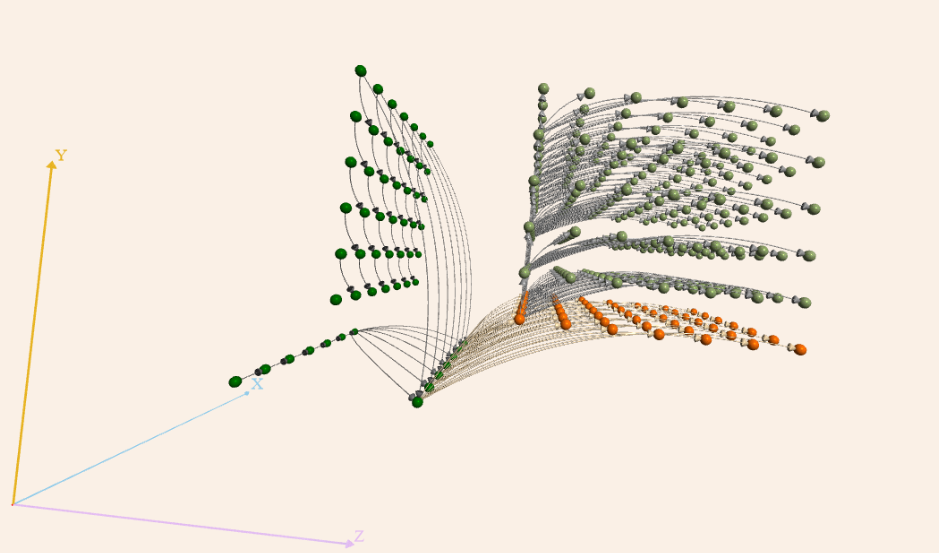
\includegraphics[scale=0.96]{lengths.png}
 \caption{Увеличение длин дуг при увеличении размерностей $n->7, m->6$}
 \label{fig:length}
\end{center}
\end{figure}

Таким образом, более правильным ответом на вопрос о количестве длинных дуг считаю $\mathbf{n}$=5.\footnote{Этот факт опирается только на приведённые рассуждения. В приложенном к заданию примере отчёта не содержится достаточно информации для однозначного определения количества длинных дуг. Т.к. в отчёте пример программы не содержит возникающих дуг при увеличении размерности с таким же типом, как в предложенном для анализа здесь.}
Если считать зависимости вида $length(dim) = const(dim), \, \forall dim \in \mathbf{N}$, где $const(dim)$ -- константы, однозначно определённая размерностью входящими в определение зависимости длины от размерности, то верный ответ = $n + n + n^2 + n^2 (m - 1) = 2n + n^2m$.
\end{packed_enum}

\section{Разметка параллельных циклов}
Поскольку условия задания не предусматривают изменения данного фрагмента, то разметка на параллельные циклы проводится только по ресурсу параллелизма, доступному в данном фрагменте.
Размеченный фрагмент приведён в листинге \ref{code:list3}.
\lstinputlisting[language=C, style=customc, label={code:list3}]{../code/pragma_program_106.c}{}
\section{Выводы}
(Почти все дальнейшие рассуждения выходят за рамки обязательного задания. Поэтому для ускорения проверки можно их пропустить, но хотелось бы узнать, если будет возможность, на сколько рассуждения верны)
\begin{enumerate}
 \item Оценим возможную степень параллелизма данного фрагмента. Доля последовательных операция равна $\alpha = \frac{n + nm + nm + 1}{n(nm + m + 2)} = \frac{46}{130} \approx 0.354$(для заданных параметров)\footnote{При увеличении n и m доля стремится к 0?}. Для оценки, примем $\alpha \approx \frac{1}{n}$ (это удовлетворяет порядку предела)
 
 Тогда, по закону Амдала, $S \leq \frac{1}{\alpha + \frac{1-\alpha}{p}} \approx n$
 \item Данный фрагмент также имеет смещённый ресурс параллельности в блоке размерности 2. На практике он может быть оптимизирован.
 \item Понятия типа дуги и зависимости длины от размерности должны быть формализовано на этапе постановки задачи, иначе может получиться несоответствие результатов.
\end{enumerate}

\newpage
\begin{thebibliography}{}
\bibitem{Voevodin02} В. В. Воеводин, Вл. В. Воеводин. Параллельные вычисления Спб, изд-во "БХВ-Петербург", 2002.

\end{thebibliography}
\end{document}
